\documentclass[article]{jss}

%%%%%%%%%%%%%%%%%%%%%%%%%%%%%%
%% declarations for jss.cls %%%%%%%%%%%%%%%%%%%%%%%%%%%%%%%%%%%%%%%%%%
%%%%%%%%%%%%%%%%%%%%%%%%%%%%%%

%% almost as usual
\author{Joseph Kelly\\Harvard University \And 
             Carl Morris\\ Harvard University\And
             Hyungsuk Tak\\Harvard University }
\title{\pkg{Rgbp}: Bayesian Hierarchical Modeling and Frequentist Method Check}

%% for pretty printing and a nice hypersummary also set:
\Plainauthor{Joseph Kelly, Carl Morris, Hyung Suk Tak} %% comma-separated
\Plaintitle{Rgbp: Bayesian Hierarchical Modeling and Frequentist Method Check} %% without formatting

%% an abstract and keywords
\Abstract{Bayesian-frequentist reconciliation via Bayesian hierarchical modeling for Gaussian, Binomial, and Poisson data and frequentist method check for good coverage probability.}
\Keywords{hierarchical model, multi-level model, random effects mixed model, method check, coverage probability, normal, binomial, poisson, shrinkage, \proglang{R}}
\Plainkeywords{keywords, comma-separated, not capitalized, r} %% without formatting
%% at least one keyword must be supplied

%% publication information
%% NOTE: Typically, this can be left commented and will be filled out by the technical editor
%% \Volume{50}
%% \Issue{9}
%% \Month{June}
%% \Year{2012}
%% \Submitdate{2012-06-04}
%% \Acceptdate{2012-06-04}

%% The address of (at least) one author should be given
%% in the following format:
\Address{
  Joseph Kelly\\
  Department of Statistics\\
  Harvard University\\
  1 Oxford Street, Cambridge, MA\\
  E-mail: \email{kelly2@fas.harvard.edu}\\
  URL: \url{http://www.people.fas.harvard.edu/~kelly2/}\\

  Carl Morris\\
  Department of Statistics\\
  Harvard University\\
  1 Oxford Street, Cambridge, MA\\
  E-mail: \email{morris@fas.harvard.edu}\\

  Hyungsuk Tak\\
  Department of Statistics\\
  Harvard University\\
  1 Oxford Street, Cambridge, MA\\
  E-mail: \email{hyungsuk.tak@gmail.com}\\

}

%% It is also possible to add a telephone and fax number
%% before the e-mail in the following format:
%% Telephone: +43/512/507-7103
%% Fax: +43/512/507-2851

%% for those who use Sweave please include the following line (with % symbols):
%% need no \usepackage{Sweave.sty}

%% end of declarations %%%%%%%%%%%%%%%%%%%%%%%%%%%%%%%%%%%%%%%%%%%%%%%

\begin{document}

%% include your article here, just as usual
%% Note that you should use the \pkg{}, \proglang{} and \code{} commands.

\section[introduction]{Introduction}
%% Note: If there is markup in \(sub)section, then it has to be escape as above.
\pkg{Rgbp} uses Bayesian machinery to estimate a two-level model (a random-effects mixed model) and allows for a check of its frequentist properties via a repeated sampling procedure (which we call a ``method check"). It is found that even in small samples our procedure yields good frequency properties. Also, this package will be useful for Bayesians who want to see a non-informative reference point before and after constructing their full-Bayesian hierarchical model. For frequentists, it will provide confidence intervals of a random-effect mixed model with good repeated sampling properties.

\section[Feasible Data Types]{Three Feasible Types of Data }
This package is intended to fit a multi-level model on the group-level (or unit-level) data in which each group-level (or unit-level) observation is believed to have the Normal, Poisson, or Binomial distribution. In this section, we will introduce three specific types of feasible datasets.

\subsection{Normal: 8 School Data}
Education Testing Service conducted randomized experiments in eight separate schools and obtained this dataset. It contains the coaching effects on SAT scores ($y_{j}, j=1, \ldots, 8$) and standard errors ($se_{j}, j=1, \ldots, 8$) of eight schools obtained after an analysis of covariance adjustment (Rubin, 1981).
\begin{CodeChunk}
\begin{CodeInput}
R> y  <- c(28,  8, -3,  7, -1,  1, 18, 12)
R> se <- c(15, 10, 16, 11,  9, 11, 10, 18)
\end{CodeInput}
\end{CodeChunk}

In the original paper, each school's coaching effect has approximately Normal sampling distribution with known sampling variance, \emph{i.e.}, standard error of each school is assumed to be known or to be accurately estimated. So, it is reasonable to think that each (group-level) coaching effect is distributed as independent Normal distribution given the unknown mean $\mu_{j}$ and known standard error:  $y_{j}\vert\mu_{j}\stackrel{ind}{\sim} \textrm{Normal}(\mu_{j}, se^{2}_{j}),~ j=1, \ldots, 8$. \pkg{Rgbp} includes this dataset and can be called by typing `\code{R> data(schools)}' on \proglang{R}.

\subsection{Poisson: 31 Hospital Data}
This dataset is about the medical profiling evaluations for Coronary Artery Bypass Graft (CABG) surgeries of 31 New York hospitals conducted in 1992 (Morris and Lysy, 2012). It comprises of the number of deaths within a month of CABG surgeries in each hospital ($z_{j},~j=1, \ldots, 31$) and total number of patients receiving CABG surgeries (case load) in each hospital ($n_{j},~j=1, \ldots, 31$). The below code is an example of input based on the last ten hospital data.
\begin{CodeChunk}
\begin{CodeInput}
R> z <- c( 14,   9,  15,  13,  35,  26,  25,  20,   35,   27)
R> n <- c(593, 602, 629, 636, 729, 849, 914, 940, 1193, 1340)
\end{CodeInput}
\end{CodeChunk}


Considering the type of data, it makes sense to assume the number of deaths in each hospital has independent Poisson distribution given the unknown parameter $\lambda_{j}$: $z_{j}\vert \lambda_{j}\stackrel{ind}{\sim} \textrm{Poisson}(n_{j}\lambda_{j})$, $j=1, \ldots, 31,$ where $n_{j}$ can be interpreted as an exposure (not necessarily an interger). This dataset is also included in the package and can be called by `\code{R> data(hospital)}' on \proglang{R}.

\subsection{Binomial: 18 Baseball Data}
This dataset contains information about batting averages of 18 major league players through their first 45 official at-bats of the 1970 season (Efron and Morris, 1975). Also, it has two covariates, League and Position, showing in which league and in which position each player was playing. In this paper, we will use Position for a tutorial purpose. For convenience, we transform this variable into a binary indicator, which is 1 if a player was a outfielder and 0 otherwise. The code below shows a way to make inputs. If we have more than one covariate, for example, \code{x1} and \code{x2}, then `\code{R> x <- cbind(x1, x2)}' will be the right input of the \code{gbp} function.
\begin{CodeChunk}
\begin{CodeInput}
R> z <- c(18, 17, 16, 15, 14, 14, 13, 12, 11, 11, 10, 10, 10, 10, 10,  9,  8,  7)
R> n <- c(45, 45, 45, 45, 45, 45, 45, 45, 45, 45, 45, 45, 45, 45, 45, 45, 45, 45)
R> x <- c( 1,  1,  1,  1,  1,  0,  0,  0,  0,  1,  0,  0,  0,  1,  1,  0,  0,  0) 
\end{CodeInput}
\end{CodeChunk}
The data indicate that independent Binomial distribution is appropriate for each player's number of hits among 45 at-bats conditioning on the unknown parameter $p_{j}$: $z_{j}\vert p_{j}\stackrel{ind}{\sim} \textrm{Binomial}(n_{j}, p_{j}), ~j=1, \ldots, 18$. This dataset is also a part of the package and can be called on \proglang{R} by `\code{R> data(baseball)}'.

\section[Multi-level Structure]{Multi-level Structure}
Our multi-level model, also called a conditionally independent hierarchical model (Kass and Steffey, 1989), is a very powerful tool for exploring the hierarchical sturucture in data. For example, we can think about a district-level hierarchy (bigger population) for 8 schools, the state-level hierarchy for 31 hospitals, and the position-level hierarchy for 18 baseball players. \code{gbp}, one of functions in \pkg{Rgbp}, fits such a hierarchical model whose first-level hierarchy has a distribution of observed data and second-level (bigger population hierarchy) has a conjugate prior distribution on the first-level parameter. Users can determine one of three types of multi-level models, such as Normal-Normal, Poisson-Gamma, and Binomial-Beta, based on their datasets. 
\\

 
\subsection[Normal-Normal]{Normal-Normal}
\code{gbp} can construct a two-level Normal-Normal hierarchical model on the 8 school data. For reference,  $\sigma^{2}_{j}$ below is assumed to be known or to be accurately estimated, and subscript \emph{j} indicates \emph{j}-th school in the dataset.
\begin{equation}
y_{j}\vert \mu_{j} \stackrel{ind}{\sim}\textrm{Normal}(\mu_{j}, \sigma^{2}_{j}),
\end{equation}
\begin{equation}
\mu_{j}\vert \beta, A\stackrel{ind}{\sim}\textrm{Normal}(\mu_{0j}, A),
\end{equation}

where $\mu_{0j} =x^{T}_{j}\beta,~j=1, \ldots, 8$, $x_{j}$ is $j$-th school's covariate vector ($m\times 1$), and $m$ is the number of regression coefficients. Note that if there is no covariate then $m$ is 1 for an intercept term, making $\mu_{0j}=\mu_{0}=\beta_{0}$ for all $j$. For reference, a paramter with a zero subscript, $\mu_{0j}$, represents a mean parameter of the prior (second-level) distribution. Also,  Based on this conjugate prior distribution, it is easy to derive corresponding posterior distribution.
\begin{equation}
\mu_{j}\vert \textbf{y}, \beta, A \stackrel{ind}{\sim}\textrm{Normal}(~(1-B_{j})y_{j} + B_{j}\mu_{0j},~(1-B_{j})\sigma^{2}_{j}),
\end{equation}
where $B_{j}\equiv\frac{\sigma^{2}_{j}}{\sigma^{2}_{j} + A},~j=1, \ldots, 8$, is called a shrinkages.

\subsection[Poisson-Gamma]{Poisson-Gamma}
\code{gbp} is also able to build a Poisson-Gamma multi-level model on the 31 hospital data. Note that a constant multiplied to the notation representing Gamma distribution below is a scale and a square bracket below indicates [mean, variance] of distribution. And for notational consistency, let's define $y_{j}\equiv \frac{z_{j}}{n_{j}}$ for all $j$.
\begin{equation}
z_{j}\vert \lambda_{j} \stackrel{ind}{\sim}\textrm{Poisson}(n_{j}\lambda_{j}),
\end{equation}
\begin{equation}
\lambda_{j}\vert \beta, r\stackrel{ind}{\sim}\frac{1}{r}\textrm{Gamma}(\lambda_{0j}r)\sim \textrm{Gamma}[\lambda_{0j}, ~\frac{\lambda_{0j}}{r}],
\end{equation}

where $\log(\lambda_{0j}) =x_{j}'\beta$, and $j=1, \ldots, 31$. Immediate posterior distribution of this Poisson-Gamma model is
\begin{equation}
\lambda_{j}\vert \textbf{z}, \beta, r \stackrel{ind}{\sim}\frac{1}{r + n_{j}}\textrm{Gamma}(r\lambda_{0j} + n_{j}y_{j})\sim\textrm{Gamma}[\lambda^{\ast}_{j},~\frac{\lambda^{\ast}_{j}}{r+n_{j}}],
\end{equation}

where $\lambda^{\ast}_{j} \equiv (1-B_{j})y_{j} + B_{j}\lambda_{0j}$,  $B_{j}\equiv \frac{r}{r+n_{j}}$, and $y_{j}\equiv \frac{z_{j}}{n_{j}}$, $j=1, \ldots, 31$. 

\subsection[Binomial-Beta]{Binomial-Beta}
Binomial-Beta hierarchical model is the last model that \code{gbp} can fit. Again, a square bracket below indicates [mean, variance] of distribution.
\begin{equation}
z_{j} \vert p_{j}\stackrel{ind}{\sim}\textrm{Binomial}(n_{j}, ~p_{j}),
\end{equation}
\begin{equation}
p_{j} \vert \beta, r\stackrel{ind}{\sim}\textrm{Beta}(rp_{0j},~ r(1-p_{0j}))\sim \textrm{Beta}[p_{0j}, ~\frac{p_{0j}(1-p_{0j})}{r + 1}],
\end{equation}

where $\log(\frac{p_{0j}}{1-p_{0j}}) =x_{j}'\beta~\textrm{and}~j=1, \ldots, 18$. Then posterior distribution is
\begin{equation}
p_{j}\vert \textbf{z}, \beta, r \stackrel{ind}{\sim}\textrm{Beta}(rp_{0j}+n_{j}y_{j},~r(1-p_{0j})+n_{j}(1-y_{j})\sim\textrm{Beta}\bigg[p^{\ast}_{j},~ \frac{p^{\ast}_{j}(1-p^{\ast}_{j})}{r+n_{j}+1}\bigg],
\end{equation}
where $p^{\ast}_{j}\equiv(1-B_{j})y_{j}+B_{j}p_{0j}$, $B_{j}\equiv\frac{r}{r+n_{j}}$, and $y_{j}\equiv\frac{z_{j}}{n_{j}}$, $j=1,\ldots,18$.


\subsection[Hyper-prior Distribution]{Hyper-prior Distribution}
Hyper-prior distribution indicates a distribution of the second-level parameters, which plays an important role in deriving a full posterior distribution of all the parameters. \code{gbp} sets a non-informative distribution on second-level parameters to let the data speak more about their estimation.
\begin{equation}
\beta \sim \textrm{Uniform on}~ \mathbf{R}^{m},~~A ~(\textrm{or}~ \frac{1}{r})\sim \textrm{Uniform}(0, \infty),
\end{equation}

where $m$ is the number of regression coefficients. For $\beta$, it is reasonable choice to take flat (non-informative) distribution because information about the location gets informative as number of groups increases. Another flat prior on the hyper-prameter $A$ (or $1/r$) that we suggest here will guarantee a posterior propriety under the moderate conditions and will give users a good repeated sampling property.
\\



\section[Estimation]{Estimation}
\subsection[Shrinkage Estimation]{Shrinkage Estimation}
Estimating shrinkage is a key part of our work because as we can see the posterior means in (3), (6), and (9) are a linear function of shrinkage and the posterior variances are also a linear (Gaussian), quadratic (Poisson), or cubic (Binomial) function of shrinkage. Once we estimate it, we can approximate the posterior moments given only data by Adam's law, for example, $E(\mu_{j}\vert \textbf{y})=E(E(\mu_{j}\vert \textbf{y}, r, A)\vert \textbf{y})$ for Gaussian model and by Eve's law, for instance, $Var(\mu_{j}\vert \textbf{y})=E(Var(\mu_{j}\vert \textbf{y}, r, A)\vert \textbf{y})+Var(E(\mu_{j}\vert \textbf{y}, r, A)\vert \textbf{y})$
\subsection[ADM]{Adjustment for Density Maximization}
When it comes to estimating a shrinkage, we can notice that it is a function of the second-level variance component, \emph{i.e.}, $B_{j}\equiv\frac{\sigma^{2}}{\sigma^{2}+A}=B_{j}(A)$ for Gaussian and $B_{j}\equiv\frac{r}{r+n_{j}}=B_{j}(r)$ for Poisson and Binomial models.
\\

In this case, one way is to obtain an MLE of the variance component with its asymptotic Normal distribution and then to use Delta method for asymptotic Normal distribution of shrinkage. But is the Normal approximation a good approximation for shrinkage that takes on a value between 0 and 1?
\\

Here the adjustment for density maximization (Morris and Tang, 2011), called ADM, comes. It assumes the Beta distribution for shrinkage, which the authors believe is a much better approximation for it, and estimates its posterior moments, \emph{i.e.}, $E(B_{j}\vert\textrm{data})$ and $Var(B_{j}\vert\textrm{data})$.

\subsection[Approximation to Posterior Distribution by Moment Matching]{Approximation to Posterior Distribution via Matching Moments}
After estimating two posterior moments, \code{gbp} reasonably approximates posterior distribution given only data, \emph{i.e.}, ($\mu_{j}\vert \textrm{data}$), ($\lambda_{j}\vert \textrm{data}$), or ($p_{j}\vert \textrm{data}$), by matching two moments with its parameters. The reason we said `reasonablely approximates' is that it is hard to find a closed form of posterior distribution given only data unless it is a Gaussian model. So, we assumed $(p_{j}\vert \textrm{data})$ had also Beta($a_{1}$, $a_{0}$) distribution and matched two estimated moments, $E(p_{j}\vert \textrm{data})$ and $Var(p_{j}\vert \textrm{data})$, with two parameters, $a_{1}$ and $a_{0}$, of this Beta distribution. 

\section[Method Check]{Method Check}
Like the two sides of the same coin, checking a statistical model always comes with fitting a model. If a fitted model cannot pass a checking process, we usually go back to the fitting process and come back to checking process iteratively. In this sense, checking a fitted model is an interactive procedure for the model justification.
\\

There are two kinds of model justification process; one is a model check and the other is a method check. The model check is for the justification of a hierarchical modeling on a specific dataset. One possible question is, ``Can this dataset benefit from such a modeling?'' Christiansen and Morris (1996) answered this question by using a mixture model, $(z_{j}\vert \beta, r)\sim\textrm{Negative-Binomial}$, for Poisson data to justify the second-level hierarchy. They found that their data had more variation than expected of the first-level Poisson distribution and Poisson hierarchical model could successfully account for such additional variation.
\\

Once we are sure that the hierarchical modeling can be appropriate for our data, the following quetsion will be about the validity of interval estimates. ``Does the confidence interval obtained via this Bayesian model-fitting process achieve pre-specified 100($1-\alpha$)\% confidence level for any true parameter values?'' Our answer is ``yes'' and \pkg{Rgbp} has a function to assure this point. From now on, all the explanations will be based on the Binomial model.

\subsection{Pseudo-data Generation Process}
Figure 1 will be helpful to understand this process. As we can see in (8), the distribution of each true parameter ($p_{j},~j=1,\ldots, 18$) depends on two hyper-parameters, $r$ and $\beta_{(m\times1)}$, where $m$ is the number of regression coefficients. Once we fix these hyper-parameters at specific values, we can generate true parameters. Suppose we sampled 500 $\textbf{p}_{(18\times1)}$'s, \emph{i.e.}, $\{\textbf{p}^{(i)}_{(18\times1)},~i=1, \ldots, 500\}$. Then, we can also generate $\{\textbf{z}^{(i)}_{(18\times1)},~i=1, \ldots, 500\}$ given each $p_{ij},$ where $i$ indicates $i$-th pseudo-dataset and $j$ does $j$-th player. Next, \code{coverage} fits the Binomial hierarchical model 500 times on $\{(\textbf{z}^{(i)}_{(18\times1)}, \textbf{n}_{(18 \times 1)}),~i=1, \ldots, 500\}$ to obtain 500*18 interval estimates. Taking the first player as an example, we have 500 pairs of ($z_{i1}$, $p_{i1}$), $i=1,\ldots, 500$, and 500 interval estimates.
\begin{figure}[h]
\begin{center}
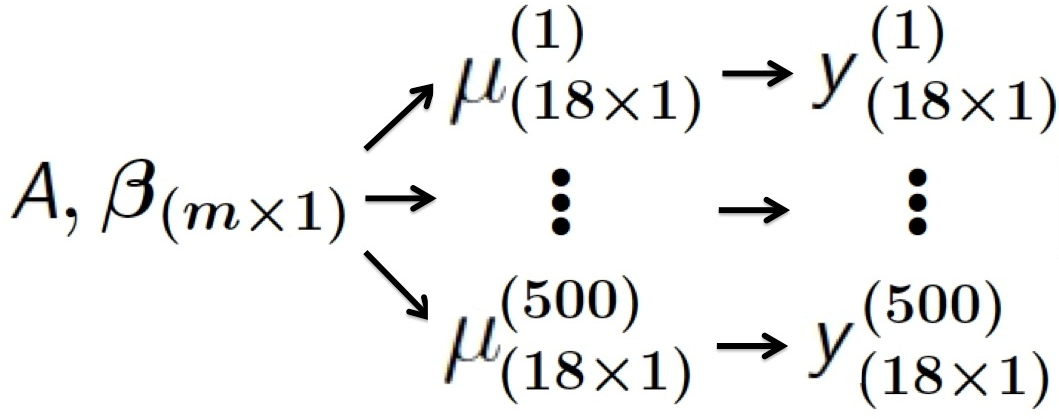
\includegraphics[width=5cm]{process.png}
\caption{Pseudo-data generating process}
\end{center}
\end{figure}

\subsection{Unbiased Coverage Probability}
Based on the generated pseudo-datasets, let's define an indicator variable, $I_{ij}$, which is 1 if $j$-th player's interval estimate from $i$-th pseudo-dataset includes $p_{ij}$ and 0 otherwise. One way to estimate the coverage probability is taking average over these indicator variables. We call it an unbiased coverage probability estimate. For example, $\bar{I}_{1}=\sum_{i=1}^{500}I_{i1}/500$ is the estimated coverage probability for the first player.

\subsection{Rao-Blackwellized Coverage Probability}
Based on the definition of Rao-Blackwellization, we define $E(I_{ij}\vert z_{ij}, r, \beta$), where $r$ and $\beta$ were fixed at first (see 5.1) and $z_{ij}$ is a sufficient statistic. This expectation is the same as Pr$(\hat{p}_{ij, low}\le p_{ij} \le\hat{p}_{ij, upp}\vert z_{ij}, r, \beta)$, where ($\hat{p}_{ij, low}$, $\hat{p}_{ij, upp}$) is $j$-th player's interval estimates (numeric values) on the $i$-th dataset. We can calculated this probability exactly because we know the distribution of $(p_{ij} \vert z_{ij}, r, \beta)$ in (9). Then, we can estimate the first player's coverage probability, for instance, by $\sum_{i=1}^{500}E(I_{i1}\vert z_{i1}, r, \beta)/500$.
\section[Example]{Example}
\subsection[Known Prior Mean]{Known Prior Mean}
\begin{figure}[h]
\begin{center}
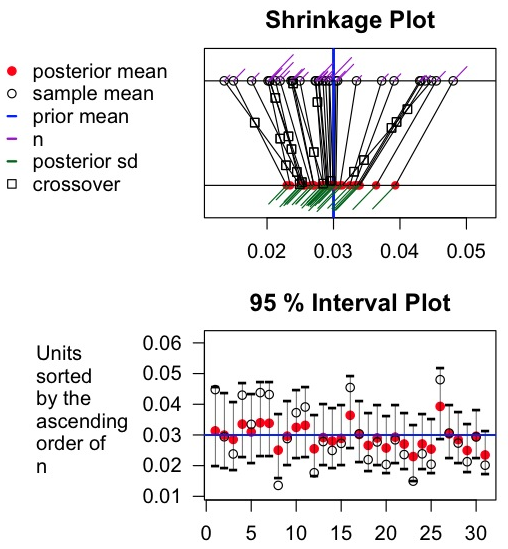
\includegraphics[scale=0.3]{hospital1.png}
\caption{Coverage and Interval Plots of \code{R> plot(p)}}
\end{center}
\end{figure}

\subsection[Unknown Prior Mean and No Covariate]{Unknown Prior Mean and No Covariate}
Using 8 school data with GR
\subsection[Unknown Prior Mean and One Covariate]{Unknown Prior Mean and One Covariate}
Using 18 baseball data with BR

\section[Discussion]{Discussion}

\section[acknowledgments]{Acknowledgments}

\section[Reference]{Reference}
1. Christiansen, C. and Morris, C. (1996). ``Fitting and Checking a Two-Level Poisson Model: Modeling Patient Mortality Rates in Heart Transplant Patients,'' in \emph{Bayesian Biostatistics}, eds. D. Berry and D. Stangl, New York: Marcel Dekker, pp. 467-561.
\\

2. Efron, B. and Morris, C. (1975). ``Data Analysis Using Stein's Estimator and its Generalizations.'' \emph{Journal of the American Statistical Association}. \textbf{70}. 311-319.
\\

3. Kass, R. and Steffey, D. (1989). ``Approximate Bayesian Inference in Conditionally Independent Hierarchical Models (Parametric
Empirical Bayes Models).'' \emph{Journal of the American Statistical Association}. \textbf{84}. 717-726.
\\

4. Morris, C. and Tang, R. (2011). ``Estimating Random Effects via Adjustment for Density Maximization.'' \emph{Statistical Science}. \textbf{26}. 271-287.
\\

5. Morris, C. and Lysy, M. (2012). ``Shrinkage Estimation in Multilevel Normal Models.'' \emph{Statistical Science}. \textbf{27}. 115-134.
\\

6. Rubin, D. B. (1981). ``Estimation in parallel randomized
  experiments.'' \emph{Journal of Educational Statistics}. \textbf{6}. 377-401.
\\


\end{document}
